\documentclass[12pt, letterpaper]{article}
\usepackage{graphicx}
\usepackage{wrapfig}
\usepackage{amsmath}
\usepackage{amsfonts}
\usepackage{geometry}
\usepackage{titlesec}
\usepackage{subfiles}
\usepackage{setspace}
\usepackage[skip=0pt, indent=0pt]{parskip}
\usepackage{float}
\usepackage{hyperref}
\usepackage{subcaption}
\usepackage{wrapfig}
\usepackage{enumitem}
\geometry{letterpaper, portrait, margin=1in}

\title{Scholarship Calculus Weekly Assignments}
\author{Phil Adams}
\date{2024}

\begin{document}

\maketitle

\begin{figure}[H]
    \centering
    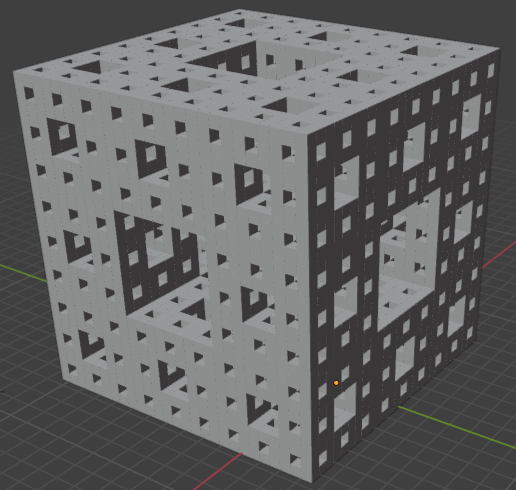
\includegraphics[width=0.5\linewidth]{images/menger.png}
\end{figure}

% Use this to change paragraph spacing throughout
\setlength{\parskip}{15pt}

These weekly assignments are intended to be challenging, and will often require you to return to them multiple times.

Do not give up! As we go through the year we will cover topics and concepts that you will either be unfamiliar with or just rusty. Treat these assignments as a chance to learn and/or get back up to speed.

\pagebreak
% Term One Questions
\newgeometry{top=10cm}
\begin{center}
    \huge
    Term One
    \normalsize
\end{center}
\restoregeometry

\pagebreak
\subfile{sections/term1week2}
\pagebreak
\subfile{sections/term1week3}
\pagebreak
\subfile{sections/term1week4}
\pagebreak
\subfile{sections/term1week5}
\pagebreak
\subfile{sections/term1week6}
\pagebreak
\subfile{sections/term1week7}
\pagebreak
\subfile{sections/term1week8}
\pagebreak
\subfile{sections/term1week9}
\pagebreak
\subfile{sections/term1week10}

\pagebreak
% Term Two Questions
\newgeometry{top=10cm}
\begin{center}
    \huge
    Term Two
    \normalsize
\end{center}
\restoregeometry

\pagebreak
\subfile{sections/term2week1}
\pagebreak
\subfile{sections/term2week2}
\pagebreak
\subfile{sections/term2week3}
\pagebreak
\subfile{sections/term2week4}
\pagebreak
\subfile{sections/term2week5}
\pagebreak
\subfile{sections/term2week6}
\pagebreak
\subfile{sections/term2week7}
\pagebreak
\subfile{sections/term2week8}

\pagebreak
% Term Three Questions
\newgeometry{top=10cm}
\begin{center}
    \huge
    Term Three
    \normalsize
\end{center}
\restoregeometry

\pagebreak
\subfile{sections/term3week1}

\pagebreak
%Answers
\newgeometry{top=10cm}
\begin{center}
    \huge
    Answers
    \normalsize
\end{center}
\restoregeometry

\pagebreak
\subfile{answers/term1week2}
\pagebreak
\subfile{answers/term1week3}
\pagebreak
\subfile{answers/term1week4}
\pagebreak
\subfile{answers/term1week5}
\pagebreak
\subfile{answers/term1week6}
\pagebreak
\subfile{answers/term1week7}
\pagebreak
\subfile{answers/term1week8}
\pagebreak
\subfile{answers/term1week9}
\pagebreak
\subfile{answers/term1week10}
\pagebreak
\subfile{answers/term2week1}
\pagebreak
\subfile{answers/term2week2}
\pagebreak
\subfile{answers/term2week3}
\pagebreak
\subfile{answers/term2week4}
\pagebreak
\subfile{answers/term2week5}
\pagebreak
\subfile{answers/term2week6}
\pagebreak
\subfile{answers/term2week7}
\pagebreak
\subfile{answers/term2week8}
\pagebreak
\subfile{answers/term3week1}
\end{document}
